% Author: Izaak Neutelings (Februari, 2020)
% page 8 https://archive.org/details/StaticAndDynamicElectricity
% https://tex.stackexchange.com/questions/56353/extract-x-y-coordinate-of-an-arbitrary-point-on-curve-in-tikz
% https://tex.stackexchange.com/questions/412899/tikz-calculate-and-store-the-euclidian-distance-between-two-coordinates

\documentclass[border=3pt,tikz]{standalone}
\usepackage{amsmath} % for \dfrac
\usepackage{bm}
\usepackage{physics}
\usepackage{tikz,pgfplots}
\usepackage[outline]{contour} % glow around text
\usetikzlibrary{angles,quotes} % for pic (angle labels)
\usetikzlibrary{decorations.markings}
\usetikzlibrary{shapes,intersections} % for path name
\tikzset{>=latex} % for LaTeX arrow head
\contourlength{1.8pt}

\usepackage{xcolor}
\colorlet{Ecol}{orange!90!black}
\colorlet{EcolFL}{orange!80!black}
\colorlet{veccol}{green!45!black}
\colorlet{EFcol}{red!60!black}
\colorlet{pluscol}{red!60!black}
\colorlet{minuscol}{blue!60!black}
\colorlet{gausscol}{green!50!black!80}
\tikzstyle{charged}=[top color=blue!20,bottom color=blue!40,shading angle=10]
\tikzstyle{charge+}=[very thin,draw=black,top color=red!80,bottom color=red!80!black,shading angle=-5]
\tikzstyle{charge-}=[very thin,draw=black,top color=blue!50,bottom color=blue!70!white!90!black,shading angle=10]
\tikzstyle{darkcharged}=[very thin,top color=blue!60,bottom color=blue!80,shading angle=10]
\tikzstyle{gauss surf}=[green!40!black,top color=green!2,bottom color=green!80!black!70,shading angle=5,fill opacity=0.6]
\tikzstyle{gauss dark}=[green!40!black,fill=green!40!black!70,fill opacity=0.8]
\tikzstyle{gauss line}=[green!40!black]
\tikzstyle{gauss dashed line}=[green!60!black!80,dashed,line width=0.2]
\tikzstyle{vector}=[->,thick,veccol]
\tikzstyle{normalvec}=[->,thick,blue!80!black!80]
\tikzstyle{EField}=[->,thick,Ecol]
\tikzstyle{EField dashed}=[dashed,Ecol,line width=0.6]
\tikzset{
  EFieldLine/.style={thick,EcolFL,decoration={markings,
                     mark=at position #1 with {\arrow{latex}}},
                     postaction={decorate}},
  EFieldLine/.default=0.5}
\tikzstyle{metal}=[top color=black!5,bottom color=black!15,shading angle=30]
\tikzstyle{measure}=[fill=green!70!black!8,midway,outer sep=0,inner sep=1]
\def\L{2.2}
\def\H{2.2}
\def\W{0.30}
\def\Nx{5}
\def\Ny{5}

%\pgfdeclareradialshading{myball}{\pgfpoint{0.5cm}{0cm}}% 
%  {rgb(0cm)=(1,1,1); rgb(0.7cm)=(0.7,0.1,0); rgb(1cm)=(0.5,0.05,0); rgb(1.05cm)=(1,1,1)}


\begin{document}


% POINT CHARGE +1
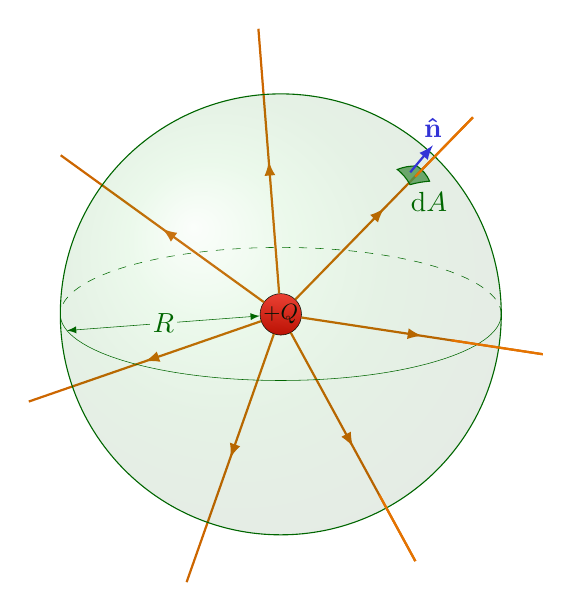
\begin{tikzpicture}
  \def\N{7}
  \def\R{2.8}
  \def\r{0.85}
  
  % SPHERE BACK
  \begin{scope}
    \clip (-\R,0) rectangle ++(2*\R,\R);
    \draw[gauss line,very thin,dashed]
      (0,0) ellipse ({\R} and {\r});
  \end{scope}
  
  % CHARGES
  \node[charge+,scale=0.8,circle,inner sep=0.27] (C) at (0,0) {$+Q$};
  
  % FIELD LINES
  \path[name path=ell](0,0) ellipse ({0.78*\R} and {\R});
  \foreach \i [evaluate={\ang=-8+\i*360/\N;}] in {1,...,\N}{
    %\message{Eline\i^^J}
    \draw[EFieldLine,name path global/.expanded=Eline\i] (C) -- ({1.2*\R*cos(\ang)},{1.3*\R*sin(\ang)}) coordinate (E\i);
    %(\ang:1.3*\R)
  }
  
  % SPHERE
  \draw[gauss line,ball color=green!70!black,fill opacity=0.1]
    (0,0) circle (2.8);
  \begin{scope}
    \clip (-\R,0) rectangle ++(2*\R,-\R);
    \draw[gauss line,very thin]
      (0,0) ellipse ({\R} and {0.3*\R});
  \end{scope}
  \draw[<->,gauss line,very thin]
    (C) -- ({\R*cos(194)},{\r*sin(194)}) node[measure] {$R$}; %{\contour{green!70!black!7}{$R$}};
  
  % VECTOR
  \draw[gauss dark,name intersections={of={Eline1} and ell,name=ES1}]
    (ES1-1) ++ (-0.081*\R,0.033*\R) to[out=20,in=180] ++(10:0.09*\R)
                                    to[out=-35,in=115] ++(-50:0.09*\R)
                                    to[out=185,in=15] ++(190:0.09*\R)
                                    to[out=120,in=-40] cycle; %node[left] {$\dd{A}$};
  \node[green!40!black,right=5,below=2] at (ES1-1) {$\dd{A}$};
  \foreach \i [evaluate={\angle=8+\i*360/\Nx;}] in {1,6,7}{
    \draw[EField,-,name intersections={of={Eline\i} and ell,name=ES\i}] (ES\i-1) -- (E\i);
  }
  \draw[normalvec] (ES1-1) ++ (138:0.03*\R) --++ (50:0.16*\R) node[above=-1] {$\vu{n}$};
  
\end{tikzpicture}


% NO CHARGE
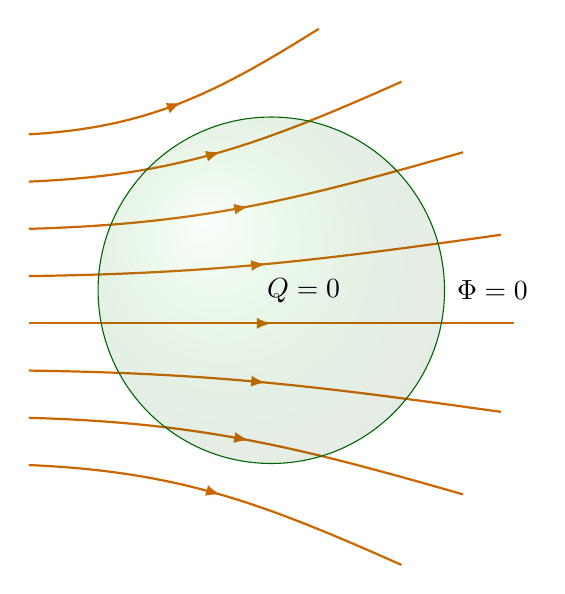
\begin{tikzpicture}
  \def\N{8}
  \def\R{2.2}
  \def\E{6.8}
  \def\r{0.85}
  
  %% CHARGES
  %\node[charge+,scale=0.8,circle,inner sep=0.24] (C) at (0,0) {$+q$};
  
  % FIELD LINES
  \path[name path=ell](0,0) ellipse ({0.78*\R} and {\R});
  \foreach \i [evaluate={
      \y=0.6*(\i-0.7-\N/2);
      \ang=5*(\i-\N/2);
      \out=0.8*(\i-\N/2);
      \in=180+8*(\i-\N/2);
      \r=2.8*\R-0.14*(\i-\N/2)^2;}] in {1,...,\N}{
    \draw[EFieldLine] (-1.4*\R,\y) to[out=\out,in=\in]++ (\ang:\r); %to[out=\out,in=\in]
  }
  
  % SPHERE
  \draw[gauss line,ball color=green!70!black,fill opacity=0.1]
    (0,0) circle (\R);
  
  % CHARGE
  \node[right=-5] at (0,0) {$Q = 0$};
  \node[right=1] at (\R,0) {$\Phi = 0$};
  
\end{tikzpicture}


% SOLID CHARGED SPHERE 3D
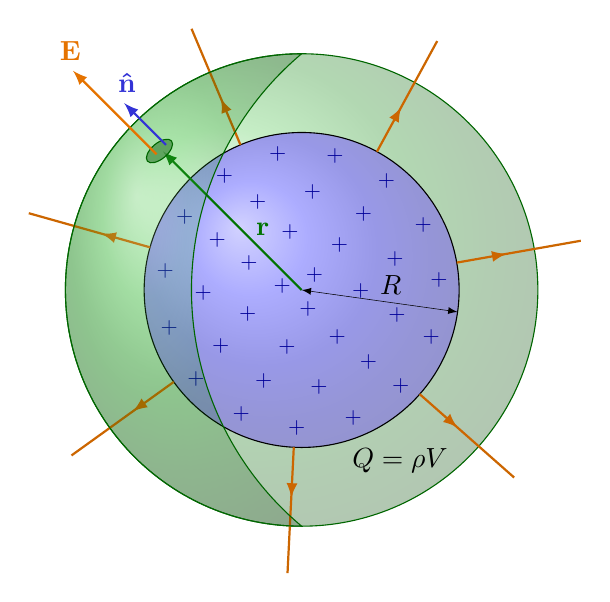
\begin{tikzpicture}
  \def\NQ{4} %13}
  \def\NE{7}
  \def\R{2.0}
  \def\r{3.0}
  \def\dtheta{50}
  \def\angle{135}
  \coordinate (P) at (\angle:0.83*\r);
  
  % SPHERE
  \draw[gauss line,ball color=green!70!black,fill opacity=0.3]
    (0,0) circle (\r);
  \fill[blue!20]
    (0,0) circle (\R);
  \draw[ball color=blue!80,fill opacity=0.3]
    (0,0) circle (\R);
  \draw[<->,black,very thin]
    (0,0) -- (-8:\R) node[midway,right=4,above=-1,black] {$R$};
  \draw[vector]
    (0,0) -- (P) node[midway,right=11,above=-9] {$\vb{r}$};
  \node at (-60:1.25*\R) {$Q = \rho V$};
  
  % CHARGES
  \foreach \i [evaluate={\rc=(\i-0.5)*\R/\NQ; \N=-1+4*\i;}] in {1,...,\NQ}{
    \foreach \j [evaluate={\ang=48+1*\i+\j*360/\N;}] in {1,...,\N}{
      \node[minuscol,scale=0.8] at (\ang:\rc) {$+$};
    }
  }
  
  % FIELD LINES
  \foreach \i [evaluate={\ang=10+\i*360/\NE;}] in {1,...,\NE}{
    \draw[EFieldLine=0.4] (\ang:\R) -- (\ang:1.2*\r);
  }
  
  % GAUSS FRONT
  \draw[gauss line,ball color=green!70!black,fill opacity=0.2]
    (0,\r) arc (90:270:\r) arc (180+\dtheta:180-\dtheta:{\r/sin(\dtheta)});
  
  % AREA ELEMENT
  \draw[gauss dark,rotate=40] (P) ++ (\angle:0.015*\r) ellipse (0.2 and 0.1);
  \draw[->,normalvec] (P) ++ (\angle-70:0.03*\r) --++ (\angle:0.25*\r) node[right=1,above] {$\vu{n}$};
  \draw[->,EField] (P) ++ (\angle+70:0.03*\r) --++ (\angle:0.5*\r) node[left=1,above] {$\vb{E}$};
  
\end{tikzpicture}


% SOLID CHARGED SPHERE 2D
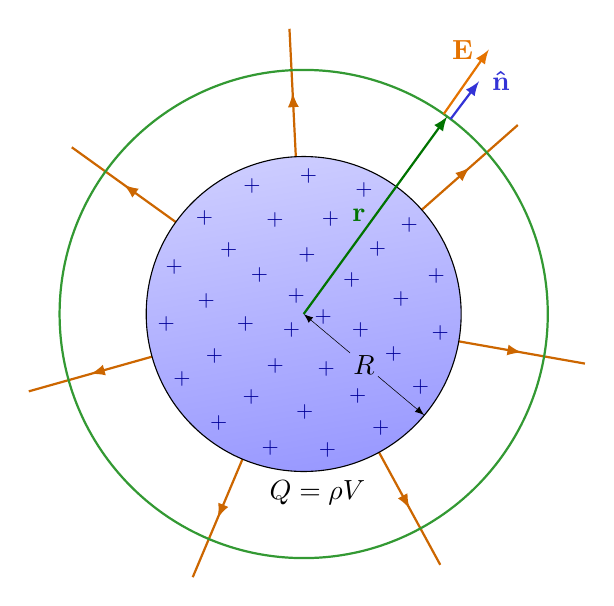
\begin{tikzpicture}
  \def\NE{7}
  \def\NQ{4}
  \def\R{2.0}
  \def\r{3.1}
  
  % FIELD LINES
  \foreach \i [evaluate={\ang=-10+\i*360/\NE;}] in {1,...,\NE}{
    \draw[EFieldLine] (\ang:\R) -- (\ang:1.17*\r);
  }
  
  % SPHERE
  \draw[charged]
    (0,0) circle (\R);
  \draw[gausscol,thick]
    (0,0) circle (\r);
  
  % CHARGES
  \foreach \i [evaluate={\rc=(\i-0.5)*\R/\NQ; \N=-1+4*\i;}] in {1,...,\NQ}{
    \foreach \j [evaluate={\ang=-8*\i+\j*360/\N;}] in {1,...,\N}{
      \node[minuscol,scale=0.8] at (\ang:\rc) {$+$};
    }
  }
  
  % VECTORS
  \node[inner sep=1] (R) at (-40:\R/2) {$R$};
  \draw[<-,very thin] (0,0) -- (R);
  \draw[->,very thin] (R) -- (-40:\R);
  \node[below=0] at (-85:\R) {$Q = \rho V$}; %fill=white,inner sep=1,
  \draw[vector] (0,0) -- (54:\r) node[midway,left=6,above=-6] {$\vb{r}$};
  \draw[EField] (55:\r) --++ (55:0.5*\R) node[left=2] {$\vb{E}$};
  \draw[normalvec] (53:\r) --++ (53:0.3*\R) node[right=1] {$\vu{n}$};
  
\end{tikzpicture}


% HOLLOW CHARGED SPHERE 2D
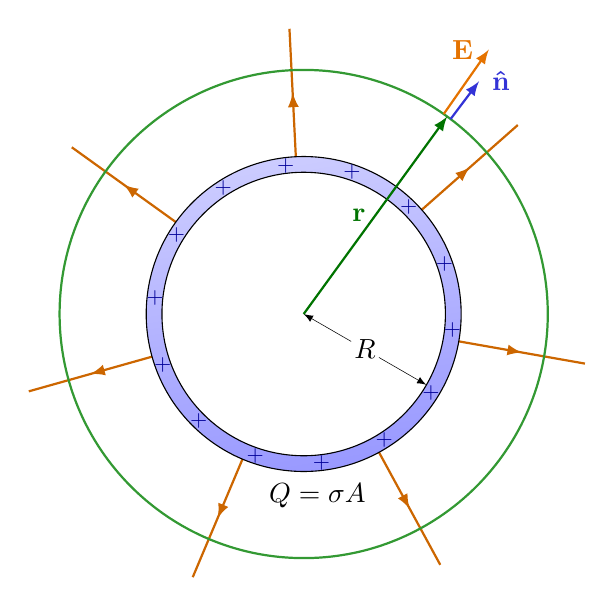
\begin{tikzpicture}
  \def\NE{7}
  \def\NQ{14}
  \def\Rin{1.80}
  \def\Rout{2.0}
  \def\r{3.1}
  
  % FIELD LINES
  \foreach \i [evaluate={\ang=-10+\i*360/\NE;}] in {1,...,\NE}{
    \draw[EFieldLine] (\ang:\Rout) -- (\ang:1.17*\r);
  }
  
  % SPHERE
  \draw[charged,even odd rule]
    (0,0) circle (\Rin) circle (\Rout);
  \draw[gausscol,thick]
    (0,0) circle (\r);
  
  % CHARGES
  \foreach \i [evaluate={\ang=-6+\i*360/\NQ;}] in {1,...,\NQ}{
    \node[minuscol,scale=0.8] at (\ang:{(\Rin+\Rout)/2}) {$+$};
  }
  
  % VECTORS
  \node[inner sep=1] (R) at (-30:\Rin/2) {$R$};
  \draw[<-,very thin] (0,0) -- (R);
  \draw[->,very thin] (R) -- (-30:\Rin);
  \node[below=1] at (-85:\Rout) {$Q = \sigma A$}; %fill=white,inner sep=1,
  \draw[vector] (0,0) -- (54:\r) node[midway,left=6,above=-6] {$\vb{r}$};
  \draw[EField] (55:\r) --++ (55:0.5*\Rout) node[left=2] {$\vb{E}$};
  \draw[normalvec] (53:\r) --++ (53:0.3*\Rout) node[right=1] {$\vu{n}$};
  
\end{tikzpicture}


% CONDUCTOR gaussian surface on outside
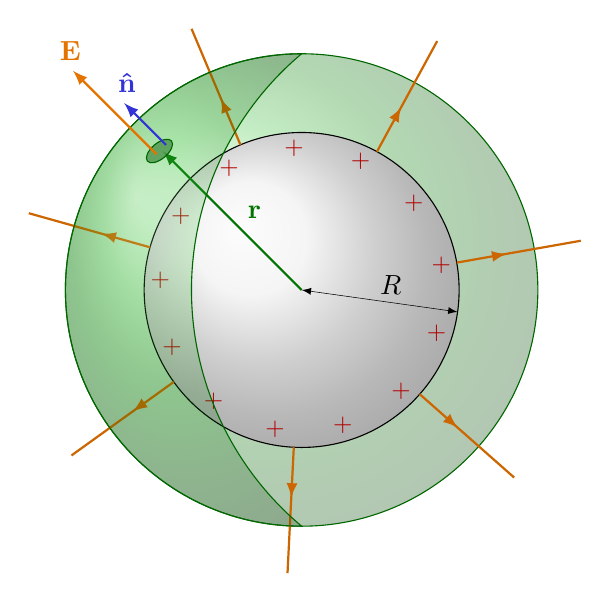
\begin{tikzpicture}
  \def\NQ{13}
  \def\NE{7}
  \def\R{2.0}
  \def\r{3.0}
  \def\dtheta{50}
  \def\angle{135}
  \coordinate (P) at (\angle:0.83*\r);
  
  % SPHERE
  \draw[gauss line,ball color=green!70!black,fill opacity=0.3]
    (0,0) circle (\r);
  \fill[white]
    (0,0) circle (\R);
  \draw[ball color=black!10,fill opacity=0.5]
    (0,0) circle (\R);
  \draw[<->,black,very thin]
    (0,0) -- (-8:\R) node[midway,right=4,above=-1,black] {$R$};
  \draw[vector]
    (0,0) -- (P) node[midway,right=8,above=-3] {$\vb{r}$};
  
  % CHARGES
  \foreach \i [evaluate={\ang=10+\i*360/\NQ;}] in {1,...,\NQ}{
    \node[red!70!black,scale=0.9] at (\ang:0.9*\R) {$+$};
  }
  
  % FIELD LINES
  \foreach \i [evaluate={\ang=10+\i*360/\NE;}] in {1,...,\NE}{
    \draw[EFieldLine=0.4] (\ang:\R) -- (\ang:1.2*\r);
  }
  
  % GAUSS FRONT
  \draw[gauss line,ball color=green!70!black,fill opacity=0.2]
    (0,\r) arc (90:270:\r) arc (180+\dtheta:180-\dtheta:{\r/sin(\dtheta)});
  
  % AREA ELEMENT
  \draw[gauss dark,rotate=40] (P) ++ (\angle:0.015*\r) ellipse (0.2 and 0.1);
  \draw[->,normalvec] (P) ++ (\angle-70:0.03*\r) --++ (\angle:0.25*\r) node[right=1,above] {$\vu{n}$};
  \draw[->,EField] (P) ++ (\angle+70:0.03*\r) --++ (\angle:0.5*\r) node[left=1,above] {$\vb{E}$};
  
\end{tikzpicture}


% CONDUCTOR gaussian surface on inside
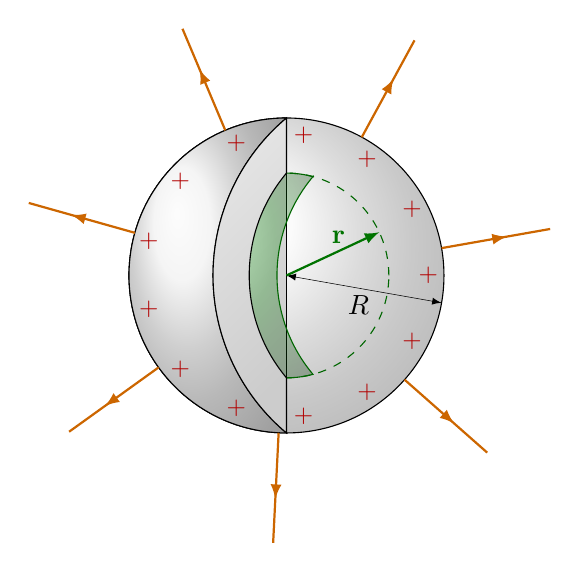
\begin{tikzpicture}
  \def\NQ{13}
  \def\NE{7}
  \def\R{2.0}
  \def\r{1.3}
  \def\dthetaI{40}
  \def\dthetaII{50}
  \def\dthetaIII{15}
  \def\angle{135}
  \coordinate (P) at (\angle:0.83*\r);
  
  % SPHERE
  \fill[white]
    (0,0) circle (\R);
  \draw[ball color=black!5,fill opacity=0.4]
    (0,0) circle (\R);
  
  % GAUSSIAN SURFACE
  \draw[top color=black!10,bottom color=black!20,shading angle=45,line width=0.2]
    (90:\R) arc (90:270:\R) -- (-90:\R) -- cycle;
  \draw[gauss line,dashed,fill opacity=0.4]
    (0,0) circle (\r);
  \draw[gauss line,ball color=green!70!black,fill opacity=0.3]
    %(0,0) circle (\r);
    (90-\dthetaIII:\r) arc (90-\dthetaIII:270+\dthetaIII:\r) arc (180+\dthetaI:180-\dthetaI:{\r*cos(\dthetaIII)/sin(\dthetaI)}) -- cycle;
  
  % VECTORS
  \draw[<->,black,very thin]
    (0,0) -- (-10:\R) node[midway,left=2,below=-1,black] {$R$};
  \draw[vector]
    (0,0) -- (25:\r) node[midway,right=2,above=0] {$\vb{r}$};
  
  % CONDUCTOR FRONT
  \fill[white]
    (0,\R) arc (90:270:\R) arc (180+\dthetaII:180-\dthetaII:{\R/sin(\dthetaII)});
  \draw[ball color=black!10,fill opacity=0.5]
    (0,\R) arc (90:270:\R) arc (180+\dthetaII:180-\dthetaII:{\R/sin(\dthetaII)});
  \draw[top color=black!10,bottom color=black!20,shading angle=45]
    (90:\R) arc (180-\dthetaII:180+\dthetaII:{\R/sin(\dthetaII)}) --
    (-90:\r) arc (180+\dthetaI:180-\dthetaI:{\r/sin(\dthetaI)}) -- cycle;
  
  % CHARGES
  \foreach \i [evaluate={\ang=0+\i*360/\NQ;}] in {1,...,\NQ}{
    \node[red!70!black,scale=0.9] at (\ang:0.9*\R) {$+$};
  }
  
  % FIELD LINES
  \foreach \i [evaluate={\ang=10+\i*360/\NE;}] in {1,...,\NE}{
    \draw[EFieldLine=0.6] (\ang:\R) -- (\ang:1.7*\R);
  }
  
\end{tikzpicture}


% CONDUCTOR with cavity
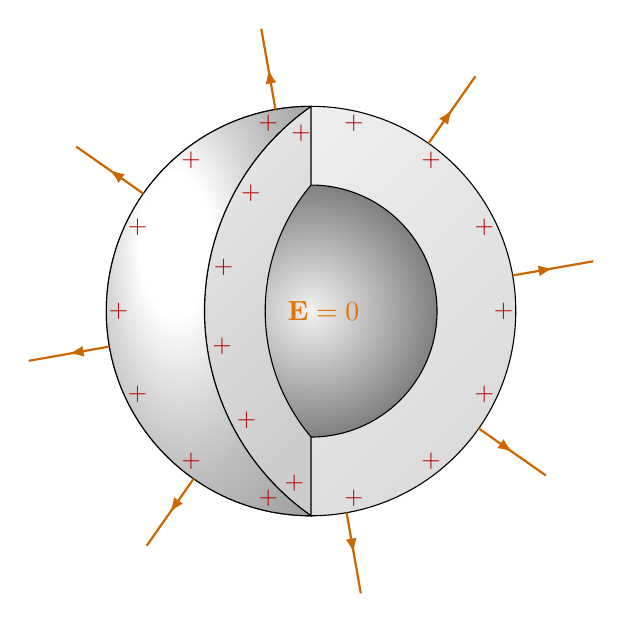
\begin{tikzpicture}
  \def\NQout{14}
  \def\NQin{14}
  \def\NQsideout{6}
  \def\NQsidein{6}
  \def\NE{8}
  \def\Rin{1.6}
  \def\Rout{2.6}
  \def\r{1.3}
  \def\E{1.4*\Rout}
  \def\dthetain{40}
  \def\dthetaout{55}
  \def\angle{135}
  %\coordinate (P) at (\angle:0.83*\r);
  
  % BACK
  \draw[top color=black!5,bottom color=black!14,shading angle=45]
    (0,0) circle (\Rout);
  \fill[white]
    (0,0) circle (\Rin);
  \draw[outer color=black!99,inner color=black!10,fill opacity=0.5] %ball color=white,fill opacity=1]
    (0,0) circle (\Rin);
  \node[Ecol,right=-12] at (0,0) {$\vb{E}=0$};
  
  % OUTSIDE FRONT
  \draw[top color=black!10,bottom color=black!20,shading angle=45]
    (90:\Rin) arc (180-\dthetain:180+\dthetain:{\Rin/sin(\dthetain)}) --
    (-90:\Rout) arc (180+\dthetaout:180-\dthetaout:{\Rout/sin(\dthetaout)}) -- cycle;
  \fill[white]
    (90:\Rout) arc (90:270:\Rout) arc (180+\dthetaout:180-\dthetaout:{\Rout/sin(\dthetaout)});
  \draw[ball color=white,fill opacity=0.5]
    (90:\Rout) arc (90:270:\Rout) arc (180+\dthetaout:180-\dthetaout:{\Rout/sin(\dthetaout)});
  
  % CHARGES
  \foreach \i [evaluate={\ang=0+\i*360/\NQout;}] in {1,...,\NQout}{
    \node[red!70!black,scale=0.9] at (\ang:0.94*\Rout) {$+$};
  }
  \foreach \i [evaluate={\ang=(180-\dthetaout)+(\i-0.7)*2.1*\dthetaout/\NQsideout;}] in {1,...,\NQsideout}{
    \node[red!70!black,shift={({\Rout/tan(\dthetaout)},0)},scale=0.9] at (\ang:{0.94*\Rout/sin(\dthetaout)}) {$+$};
  }
  \foreach \i [evaluate={\ang=10+\i*360/\NE;}] in {1,...,\NE}{
    \draw[EFieldLine=0.5] (\ang:\Rout) -- (\ang:\E);
  }
  
\end{tikzpicture}


% CONDUCTOR with cavity
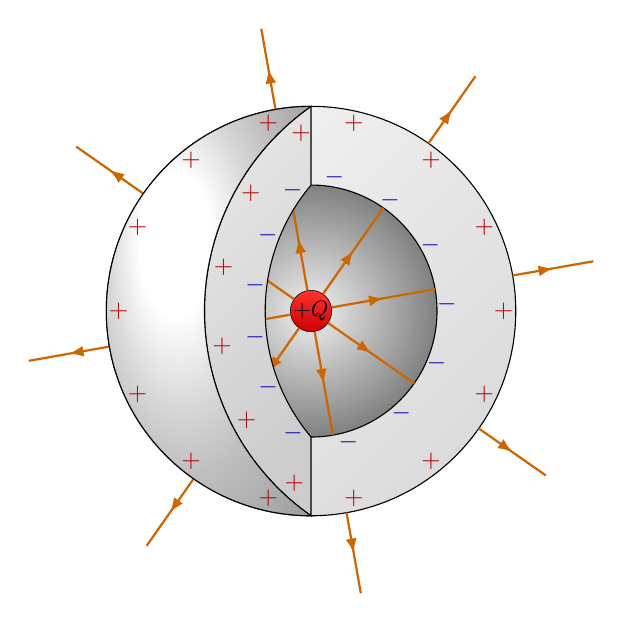
\begin{tikzpicture}
  \def\NQout{14}
  \def\NQin{14}
  \def\NQsideout{6}
  \def\NQsidein{6}
  \def\NE{8}
  \def\Rin{1.6}
  \def\Rout{2.6}
  \def\r{1.3}
  \def\E{1.4*\Rout}
  \def\dthetain{40}
  \def\dthetaout{55}
  \def\angle{135}
  %\coordinate (P) at (\angle:0.83*\r);
  
  % BACK
  \draw[top color=black!5,bottom color=black!14,shading angle=45]
    (0,0) circle (\Rout);
  \fill[white]
      (0,0) circle (\Rin);
  \draw[outer color=black!99,inner color=black!10,fill opacity=0.5] %ball color=white,fill opacity=1]
      (0,0) circle (\Rin);
  
  % INSIDE CHARGE
  \node[charge+,scale=0.8,circle,inner sep=0.27] (Q) at (0,0) {$+Q$};
  \foreach \i [evaluate={\ang=10+\i*360/\NE;}] in {1,...,\NE}{
    \draw[EFieldLine=0.5] (Q) -- (\ang:\Rin);
    \draw[EFieldLine=0.5] (\ang:\Rout) -- (\ang:\E);
  }
  
  % CHARGES INSIDE
  \foreach \i [evaluate={\ang=3+\i*360/\NQin;}] in {1,...,\NQin}{
    \node[blue!70!black,scale=0.9] at (\ang:1.08*\Rin) {$-$};
  }
  
  % OUTSIDE FRONT
  \draw[top color=black!10,bottom color=black!20,shading angle=45]
    (90:\Rin) arc (180-\dthetain:180+\dthetain:{\Rin/sin(\dthetain)}) --
    (-90:\Rout) arc (180+\dthetaout:180-\dthetaout:{\Rout/sin(\dthetaout)}) -- cycle;
  \fill[white]
    (90:\Rout) arc (90:270:\Rout) arc (180+\dthetaout:180-\dthetaout:{\Rout/sin(\dthetaout)});
  \draw[ball color=white,fill opacity=0.5]
    (90:\Rout) arc (90:270:\Rout) arc (180+\dthetaout:180-\dthetaout:{\Rout/sin(\dthetaout)});
  
  % CHARGES
  \foreach \i [evaluate={\ang=0+\i*360/\NQout;}] in {1,...,\NQout}{
    \node[red!70!black,scale=0.9] at (\ang:0.94*\Rout) {$+$};
  }
  \foreach \i [evaluate={\ang=(180-\dthetain)+(\i-0.7)*2.15*\dthetain/\NQsidein;}] in {1,...,\NQsidein}{
    \node[blue!70!black,shift={({\Rin/tan(\dthetain)},0)},scale=0.9] at (\ang:{1.06*\Rin/sin(\dthetain)}) {$-$};
  }
  \foreach \i [evaluate={\ang=(180-\dthetaout)+(\i-0.7)*2.1*\dthetaout/\NQsideout;}] in {1,...,\NQsideout}{
    \node[red!70!black,shift={({\Rout/tan(\dthetaout)},0)},scale=0.9] at (\ang:{0.94*\Rout/sin(\dthetaout)}) {$+$};
  }
  
\end{tikzpicture}



\end{document}
